% Created 2021-05-11 Tue 07:10
% Intended LaTeX compiler: pdflatex
\documentclass{beamer}\usepackage{listings}
\usepackage{color}
\usepackage{amsmath}
\usepackage{array}
\usepackage[T1]{fontenc}
\usepackage{natbib}
\lstset{
keywordstyle=\color{blue},
commentstyle=\color{red},stringstyle=\color[rgb]{0,.5,0},
literate={~}{$\sim$}{1},
basicstyle=\ttfamily\small,
columns=fullflexible,
breaklines=true,
breakatwhitespace=false,
numbers=left,
numberstyle=\ttfamily\tiny\color{gray},
stepnumber=1,
numbersep=10pt,
backgroundcolor=\color{white},
tabsize=4,
keepspaces=true,
showspaces=false,
showstringspaces=false,
xleftmargin=.23in,
frame=single,
basewidth={0.5em,0.4em},
}
\usepackage{natbib, dsfont, pgfpages, tikz,amssymb, amsmath,xcolor}
\bibliographystyle{abbrvnat}
% New operators and commands
\newcommand{\Z}{\mathbb{Z}}
\newcommand{\Q}{\mathbb{Q}}
\newcommand{\R}{\mathbb{R}}
\newcommand{\N}{\mathbb{N}}
\newcommand{\C}{\mathbb{C}}
\renewcommand{\S}{\mathbb{S}}
\newcommand{\blank}{\makebox[1ex]{\textbf{$\cdot$}}}
\newcommand\independent{\protect\mathpalette{\protect\independenT}{\perp}}
\def\independenT#1#2{\mathrel{\rlap{$#1#2$}\mkern2mu{#1#2}}}
\renewcommand{\phi}{\varphi}
\renewcommand{\epsilon}{\varepsilon}
\newcommand*\diff{\mathop{}\!\mathrm{d}}
\newcommand{\weakly}{\rightsquigarrow}
\newcommand\smallO{
  \mathchoice
    {{\scriptstyle\mathcal{O}}}% \displaystyle
    {{\scriptstyle\mathcal{O}}}% \textstyle
    {{\scriptscriptstyle\mathcal{O}}}% \scriptstyle
    {\scalebox{.6}{$\scriptscriptstyle\mathcal{O}$}}%\scriptscriptstyle
}
\newcommand{\midd}{\; \middle|\;}
\newcommand{\1}{\mathds{1}}
\usepackage{ifthen} %% Empirical process with default argument
% \newcommand{\G}[1][]{%
%    \ifthenelse{ \equal{#1}{} }
%       {\ensuremath{\mathbb{G}_n}}
%       {\ensuremath{\mathbb{G}_{#1}}}
% }
% New version:
\newcommand{\G}[2][n]{
{\ensuremath{\mathbb{G}_{#1}}{\left[#2\right]}}
}
\DeclareMathOperator*{\argmin}{\arg\!\min}

% New operators for consistent notation
\newcommand{\V}{\mathrm{Var}} % variance
\newcommand{\measure}[1]{\mathrm{{#1}}} % measure
% \newcommand{\measure}[1]{\textnormal{\textbf{{#1}}}} % measure
\newcommand{\m}[1]{\measure{#1}} % measure shortcut
\newcommand{\eqd}{\stackrel{d}{=}} % equality in distribution
\newcommand{\arrowP}{\xrightarrow{\; \m{P} \;}} % convergence in probability
\newcommand{\leb}{\lambda} % the Lebesgue measure
\newcommand{\T}{\top} % transpose

\usepackage{xargs}
% Make it easy to change counterfactual notation:
\newcommandx{\cf}[4][3={}, 4={}]{
  % \ifthenelse{ \equal{#4}{} }
  % {{#1^{#2}}(#3)}
  {\ifthenelse{ \equal{#3}{} }
    {{#1^{#2}}_{#4}}
    {{#1^{#2}}_{#4}(#3)}}
}

% Easily change notation:
\DeclareMathOperator{\TT}{\Psi} % target parameter
\newcommand{\lp}{\mathcal{L}_{\P}^2} % shortcut for lp2 space
\newcommand{\empmeas}{\hat{\mathbb{P}}_n} % empirical measure
\DeclareMathOperator{\E}{\mathbb{E}} % expectation
\renewcommand{\P}{\m{P}} % probability
\newcommand{\ic}{\mathrm{IF}} % influence curve
\setbeamertemplate{footline}[frame number]
\beamertemplatenavigationsymbolsempty
\usepackage{appendixnumberbeamer}
\setbeamercolor{gray}{bg=white!90!black}

\renewcommand*\familydefault{\sfdefault}
\itemsep2pt
\usepackage[utf8]{inputenc}
\usepackage[T1]{fontenc}
\usepackage{graphicx}
\usepackage{grffile}
\usepackage{longtable}
\usepackage{wrapfig}
\usepackage{rotating}
\usepackage[normalem]{ulem}
\usepackage{amsmath}
\usepackage{textcomp}
\usepackage{amssymb}
\usepackage{capt-of}
\usepackage{hyperref}
\usetheme{default}
\author{Anders Munch}
\date{May 11, 2021}
\title{Influence functions and functional derivatives}
\begin{document}

\maketitle
\begin{frame}{Outline}
\tableofcontents
\end{frame}

\section{Setting}
\label{sec:org95084f7}
\begin{frame}[label={sec:org61f5255}]{Disclaimer}
\begin{itemize}[<+->]
\item The note is work in progress, and we have not used it before -- you are very welcome to comment on
weird/unclear passages.
\item You should see it as a service -- some exact mathematical statements are collected there if you
care about it, but the important part is the intuition which we talk about today.
\item Do NOT write like this in your report!
\end{itemize}
\end{frame}
\begin{frame}[label={sec:org0637092}]{A statistical problem}
We call a collection of probability measures \(\mathcal{P}\) together with a functional \(\TT \colon
\mathcal{P} \rightarrow \R\) \emph{a statistical problem}.

\vfill

\begin{example}<2->[Average treatment effect]
We are given $n$ iid. sample of $O \sim \P$, with \alt<3>{$\P \in
  \color{red}{\mathcal{P}}$}{$\P \in \mathcal{P}$} and where \(O= (X, A, Y)\), with \(X\in \R^d\),
\(A\in \lbrace 0,1\rbrace\), and \(Y\in\lbrace 0, 1\rbrace\). We want to estimate the average
treatment effect
\begin{equation*}
  \E_{\P}\left[ f(1, X) - f(0, X) \right],  
\end{equation*}
with $f(a, x) := \E_{\P}\left[ Y \mid A=a, X=x  \right]$. The target parameter is
\begin{equation*}
  \alt<3>{{\color{red}\TT}}{\TT}(\P) =  \E_{\P}\left[ f_{\P}(1, X) - f_{\P}(0, X) \right].
\end{equation*}
\end{example}
\end{frame}

\begin{frame}[label={sec:org06ccbf7}]{Target and nuisance parameters}
\begin{description}
\item[{Target parameter}] Low-dimensional, scientifically meaningful. \pause
\item[{Nuisance parameters}] Needed to express the target parameter. \pause
\end{description}

\begin{example}[ATE]
The ATE can be written as \(\TT(\P) = \P[\phi_1] = \P[\phi_2] = \P[\phi_3]\), for
\begin{equation*}
  \begin{gathered}
    \phi_1(o; f) := f(1,x) - f(0,x), \\
    \phi_2(o; \pi) := \frac{a\,y}{\pi(x)} - \frac{(1-a)\,y}{1-\pi(x)}, \\
    \phi_3(o; f, \pi) := \phi_1(o; f) + \phi_2(o; \pi) - \frac{a\,f(1,x)}{\pi(x)} +
    \frac{(1-a)\,f(0,x)}{1-\pi(x)} 
  \end{gathered}
\end{equation*}

$\P[\phi]$ means
\begin{equation*}
  \P[\phi] = \E_{\P}\left[ \phi(O) \right] = \int \phi(o) \diff \P(o).
\end{equation*}
\end{example}
\end{frame}

\begin{frame}[label={sec:org99f4169}]{High-/infinite-dimensional nuisance parameters}
A parametric setting means that \(\mathcal{P}\) is finite-dimensional. We are interested in
\emph{nonparametric} or \emph{semiparametric} settings which mean that \(\mathcal{P}\) is
infinite-dimensional.

\vfill \pause

\begin{beamercolorbox}[rounded=true]{gray}
\centering Having our data set and scientific question in mind, why would it be of interest to use
infinite-dimensional nuisance parameters?
\end{beamercolorbox}

\vfill \pause
Trying to control for confounding \(\implies\) nice to have:
\begin{itemize}
\item flexible model
\item many covariates
\end{itemize}
\end{frame}

\section{Motivation}
\label{sec:orgfd98193}
\begin{frame}[label={sec:org0ebc9c8}]{Toy example: Integrated kernel density}
$\mathcal{P}$ consist all probability measures with continuous Lebesgue-density (this is an
infinite-dimensional space). We want to estimate $F(x) = \P(X \leq x)$ for unknown
$\P \in \mathcal{P}$. \pause Our target parameter is then $\theta = \TT(\P) = F_{\P}(x)$ which we
can express as
\begin{equation*}
  \TT(\P) = \TT_0(f) := \int_{-\infty}^x f(z) \diff z, \quad \text{for} \quad \P = f \cdot \leb,
\end{equation*}
because of our assumption about $\mathcal{P}$. \pause We want to use \textbf{machine learning} (!) for this problem,
so use a kernel estimator, i.e.,
\begin{equation*}
  \hat{f}_n(x) = \empmeas[k_h(X, x)] = \frac{1}{n}\sum_{i=1}^{n}k_h(X_i, x),
\end{equation*}
where $k_h$ is, e.g, $k_h(x,y) = g\left( \frac{x-y}{h} \right)$, with $g$ the density for the
standard Gaussian distribution, and the bandwidth $h$ is chosen using cross-validation. \pause We
then obtain the target estimator $\hat{\theta}_n = \TT_0(\hat{f}_n)$.
\end{frame}

\begin{frame}[label={sec:orgbadc79a}]{How does this work in practice?}
\pause
\begin{center}
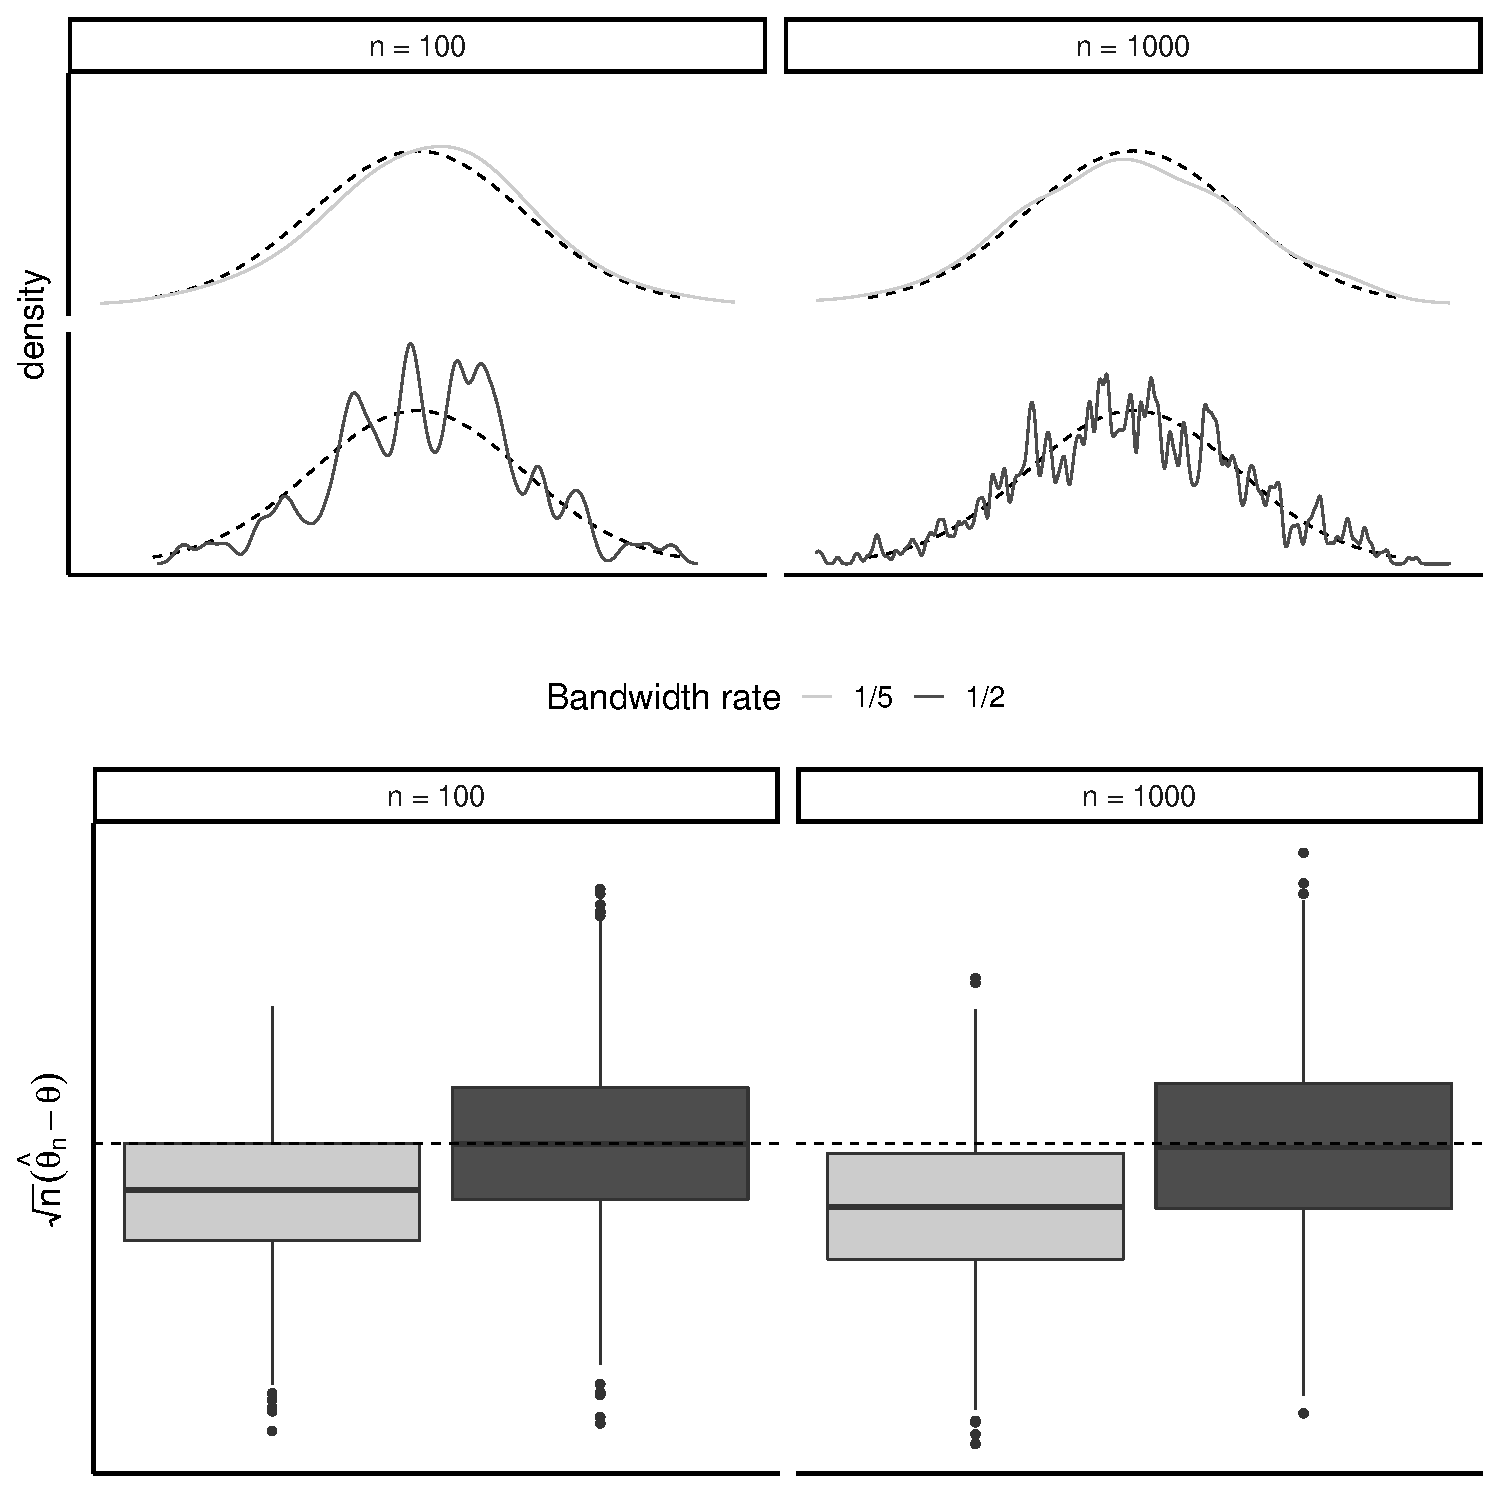
\includegraphics[width=0.75\textwidth]{./figures/kernel-undersmooth-viz-presentation-3.pdf}
\end{center}
\end{frame}

\begin{frame}[label={sec:org264b203}]{What happened?}
\pause

Consider a general problem \((\mathcal{P}, \TT)\) for which we can write \(\TT(\P) = \TT_0(\P, \nu) =
\P[\phi(O, \nu)]\). \pause We have
\begin{align*}
  \sqrt{n}
  \left(
  \hat{\theta}_n - \theta
  \right)
  & =  \sqrt{n}
    \left(
    \TT_0(\empmeas,\hat{\nu}_n) - \TT_0(\P,\nu)
    \right) \\
  & =
    \sqrt{n}
    \left(
    \empmeas[\phi(O, \hat{\nu}_n)] -
    \P[\phi(O, \nu)]
    \right) \\
  & =
    \sqrt{n}
    \left(
    \empmeas[\phi(O, \hat{\nu}_n)] 
    \pm \P[\phi(O, \hat{\nu}_n)] % + \P[\phi(O, \hat{\nu}_n)]
    - \P[\phi(O, \nu)]
    \right)    \\
  & =
    \G{\phi(O, \hat{\nu}_n) } +
    \sqrt{n} 
    \left\{
    \TT_0(\P,  \hat{\nu}_n) - \TT_0(\P,  \nu)
    \right\},
\end{align*}
with $\mathbb{G}_n: = \sqrt{n}(\empmeas -\P)$ the empirical process.

\vfill \pause

\begin{description}[<+->]
\item[{\(\G{\phi(O, \hat{\nu}_n) }\)}] determines the (main) variance
\item[{\(\TT_0(\P,  \hat{\nu}_n) - \TT_0(\P,  \nu)\)}] is bias!
\end{description}
\end{frame}

\begin{frame}[label={sec:org6c86efb}]{What to do?  -- Taylor expansion}
\pause
Assume we could make a Taylor expansion of $\nu \mapsto \TT_0(\P, \nu)$, so that
\begin{equation*}
  \TT_0(\P,  \hat{\nu}_n) - \TT_0(\P,  \nu)
  = \mathrm{D}_{\nu}{\TT_0}[\hat{\nu}_n - \nu] +
  \mathcal{O}_{\P}(\Vert \hat{\nu}_n - \nu \Vert_{\mathcal{V}}^2).
\end{equation*}
\pause The decomposition then becomes
\begin{align}
  \sqrt{n}
  \left(
  \hat{\theta}_n - \theta
  \right)
  = \; & \G{\phi( O, \hat{\nu}_n)} \\
    & + \mathrm{D_{\nu}{\TT_0}}{ \left[
      \sqrt{n}(\hat{\nu}_n - \nu)
      \right]} \\
    &  +  \mathcal{O}_{\P}(\sqrt{n}\Vert \hat{\nu}_n - \nu \Vert_{\mathcal{V}}^2).
\end{align}
\pause
\begin{enumerate}[(1)]
\item can be handled by empirical process theory or sample splitting \pause
\item is our focus! $\rightarrow$ make sense of this \pause
\item is specific to the nuisance estimator (and the functional $\TT$). Importantly, the rate
  $\sqrt{n}\Vert \hat{\nu}_n - \nu \Vert_{\mathcal{V}} = \smallO_{\P}(n^{-1/4})$ is sufficient.
\end{enumerate}
\end{frame}

\section{Functional derivatives}
\label{sec:orgc685146}
\begin{frame}[label={sec:org6e2d2cc}]{Defining a functional derivative}
\begin{block}{What is a derivative? \pause}
A linear approximation \(\dot{\TT}_x\) to the map \(\TT\) at \(x \in \mathcal{M}\), i.e.,
\begin{equation*}
  \left\Vert
    \TT(x + \epsilon_n h_n) - \TT(x) - \dot{\TT}_x(\epsilon_n h_n)
  \right\Vert = \smallO(\epsilon_n),
\end{equation*}
when \(\epsilon_n \rightarrow 0\).

\pause \hfill
\end{block}
This expression also makes sense for functionals (or operators) \(\TT\).

\pause \hfill

\begin{itemize}[<+->]
\item For which \(h_n\) should this hold? Along ``lines'', ``paths'', or ``uniformly'' (\(h_n\) fixed,
converging, or bounded)?
\item Which norm on \(\mathcal{M}\) should we use?
\item In which space should we represent \(\mathcal{P}\)?
\end{itemize}
\end{frame}

\begin{frame}[label={sec:org92ecb98}]{Pathwise Hadamard differentiability}
Think of the gradient of a function defined on a manifold (surface).

\begin{center}
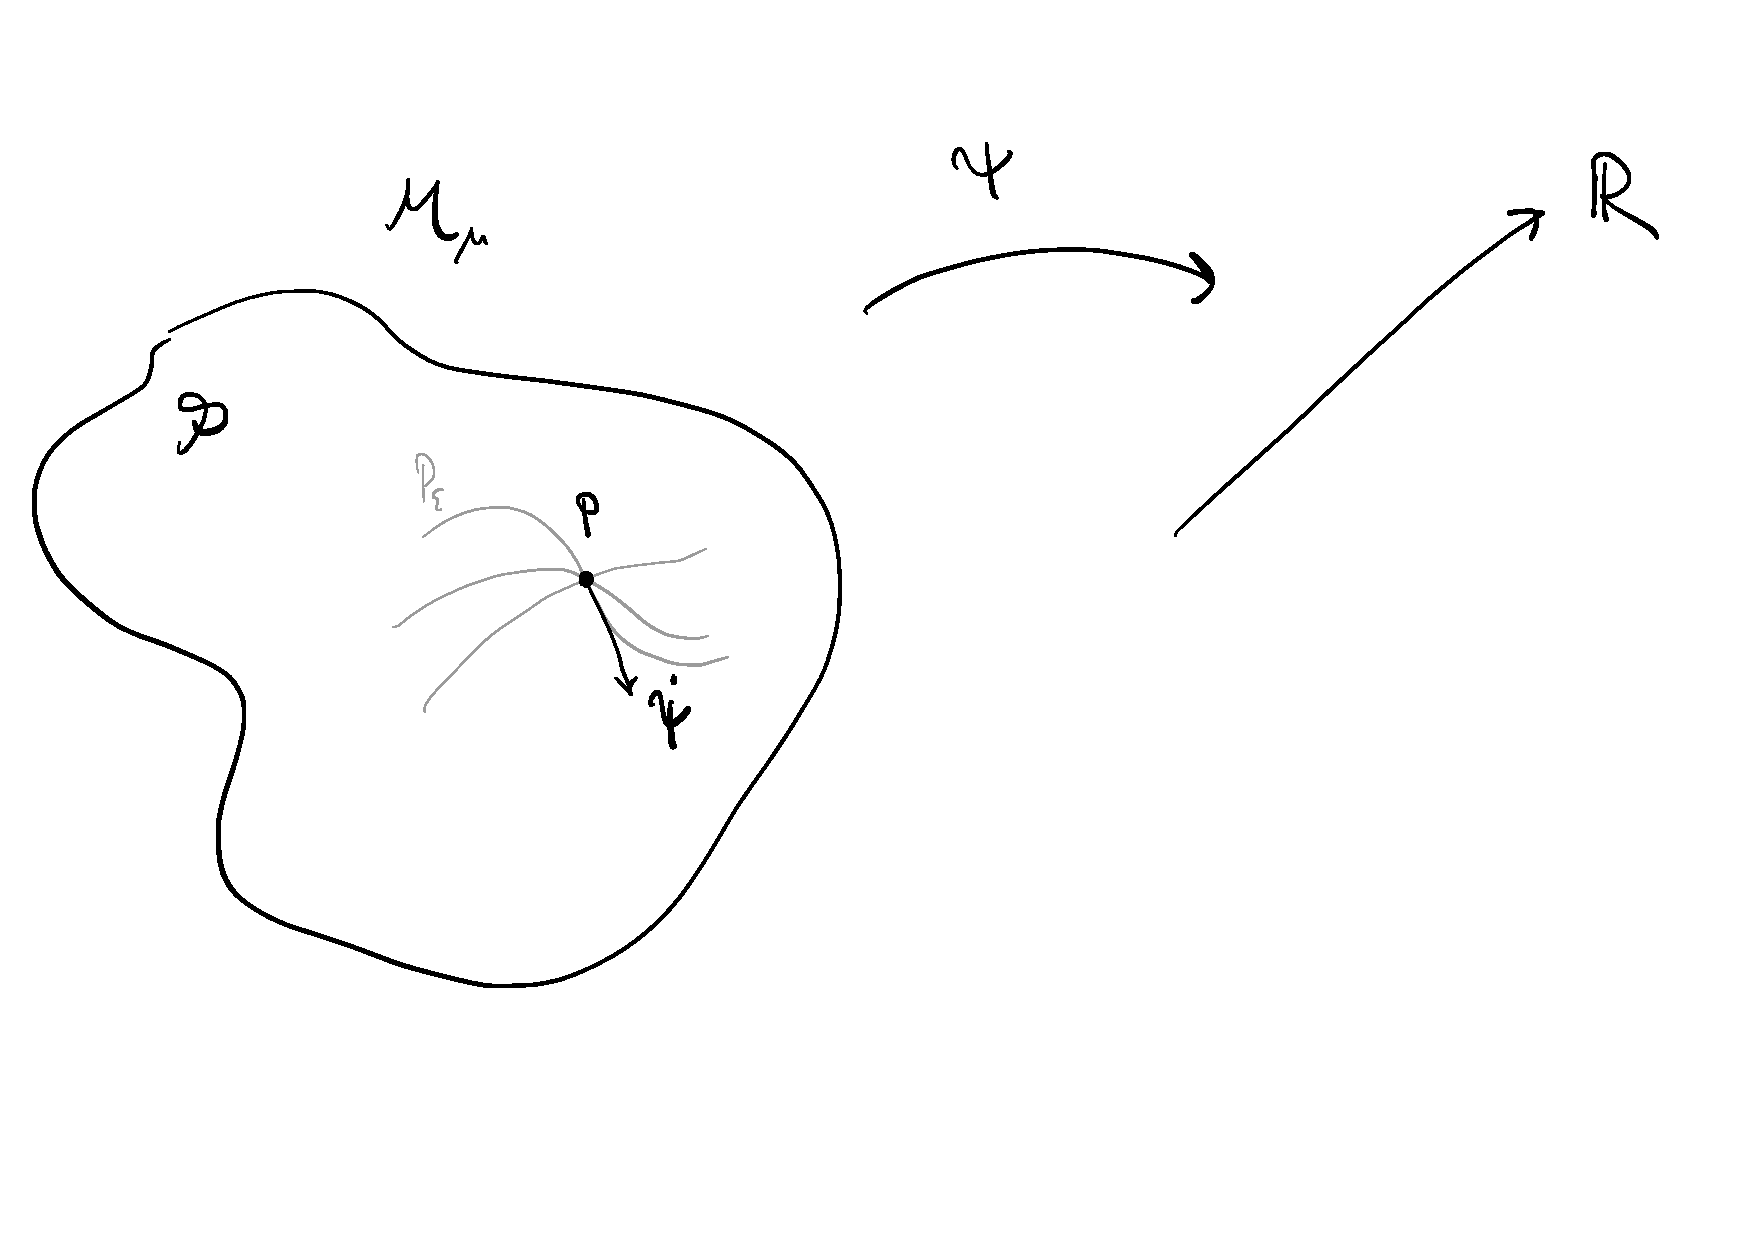
\includegraphics[width=0.9\textwidth]{./figures/pathwise-dif.pdf}
\end{center}
\end{frame}


\section{Canonical gradient / efficient influence function}
\label{sec:org4c04450}
\begin{frame}[label={sec:org2a6d59f}]{Canonical gradient}
\begin{definition}[Canonical gradient]
Let \((\mathcal{P}, \TT)\) be a statistical problem, with \(\mathcal{P} \subset \mathcal{M}_{\mu}\),
and \(\dot{\mathcal{P}}_{\P}\) the tangent space of \(\mathcal{P}\) at \(\P \in \mathcal{P}\). If
\(\TT \colon \mathcal{P} \rightarrow \R\) is Hadamard differentiable at \(\P\) tangential to
\(\dot{\mathcal{P}}_{\P}\), we refer to the Hadamard derivative \(\dot{\TT}_{\P}\) as the
\textit{canonical gradient of the statistical problem}.

\pause
\end{definition}

\begin{block}{Characterizing property}
With $\Gamma_{\P} := \overline{\mathrm{span}}\{\dot{\ell}_0\} \subset \lp$, where
$\dot{\ell}_0 = \partial_0{\log(p_{\epsilon})}$ is the score function of the sub-model
$\P_{\epsilon}$, there exists a unique element $\phi_{\P} \in \Gamma_{\P}$ such that
\begin{equation*}
  \partial_0{\TT(\P_{\epsilon})}
  = \langle \phi_{\P}, \dot{\ell}_0 \rangle_{\P}
\end{equation*}
holds for any differentiable submodel $\P_{\epsilon}$ with score function $\dot{\ell}_0$.
\end{block}
\end{frame}

\begin{frame}[label={sec:org8217328}]{Canonical gradient for the ATE}
\begin{example}[ATE]
When we make no assumptions about \(\mathcal{P}\), the canonical gradient for the ATE problem
\begin{align*}
  \phi_{\P}(o; f, \pi) := \;& f(1,x) - f(0,x) \\
                             & +  \frac{a\,y}{\pi(x)} - \frac{(1-a)\,y}{1-\pi(x)} \\
                             &  - \frac{a\,f(1,x)}{\pi(x)} +
                               \frac{(1-a)\,f(0,x)}{1-\pi(x)} \\
                             &  - \TT(\P)
\end{align*}
\pause One way to show this is to first show that the tangent space $\Gamma_{\P}$ is the full subset
$\mathbb{H}_0 \subset \lp$ of zero-mean functions, and then show that
$ \partial_0{\TT(\P_{\epsilon})} = \langle \phi_{\P}, \dot{\ell}_0 \rangle_{\P}$ for all
$\P_{\epsilon}$ (see for instance \cite{kennedy2016semiparametric}).
\end{example}
\end{frame}

\section{Summary of main results}
\label{sec:org0a1f9ac}
\begin{frame}[label={sec:org25df887}]{Neyman orthogonality}
\begin{theorem}[Neyman orthogonality]
If $\TT(\P) = \TT_0(\P, \nu) = \P[\phi(O, \nu(\P))]$ and $\phi(\blank, \nu) - \P[\phi(O, \nu)]$ is the
canonical gradient of $(\mathcal{P}, \TT)$ then $\mathrm{D_{\nu}{\TT_0}} = 0$.

\hfill \pause
\end{theorem}

\begin{block}{Debiasing}
The \emph{first order} bias, coming from \(\TT_0(\P, \hat{\nu}_n) - \TT_0(\P, \nu)\), is removed. 
\end{block}
\end{frame}

\begin{frame}[label={sec:org327e82d}]{Efficiency}
\begin{definition}[RAL estimators]
An estimator $\hat{\theta}_n$ of the parameter $\theta = \TT(\P)$ under the model $\mathcal{P}$, is
called \textit{asymptotically linear} with \textit{influence function} $\ic(\blank, \P) \in \lp$, if 
$\P[\ic(O, \P)] = 0$ for all $\P \in \mathcal{P}$, and 
\begin{equation*}
  \hat{\theta}_n - \theta = \empmeas[\ic(O, \P)] + \smallO_{\P}(n^{-1/2}).
\end{equation*}
\end{definition}

\begin{theorem}<2->[Efficient influence function]
The RAL estimator with lowest possible asymptotic variance has the canonical gradient as its
influence function.
\end{theorem}
\end{frame}

\section{Next step -- constructing estimator}
\label{sec:org53682b6}
\begin{frame}[label={sec:org94c4227}]{Constructing estimators: Solve the efficient score equation}
Find a parametrization \(\TT(\P) = \P[\phi(O, \nu)]\) such that \(\phi\) is the (canonical) gradient.
\pause Then by Neyman orthogonality and assumptions we can write
\begin{align*}
  \sqrt{n}
  \left(
  \hat{\theta}_n - \theta
  \right)
  = \; & \G{\phi( O, \hat{\nu}_n)} \uncover<4->{&& {\color{red}= \G{\phi( O, \nu)}}} \\
       & + \mathrm{D_{\nu}{\TT_0}}{ \left[
         \sqrt{n}(\hat{\nu}_n - \nu)
         \right]} \uncover<3->{&& {\color{red}= 0}}\\
       &  +  \mathcal{O}_{\P}(\sqrt{n}\Vert \hat{\nu}_n - \nu \Vert_{\mathcal{V}}^2) 
         \uncover<4->{&& {\color{red}=  \smallO_{\P}(1)}} \\[0.18cm]
  \uncover<5->{= \; & \G{\phi( O, \nu)} + \smallO_{\P}(1).}
\end{align*}
\uncover<6->{Hence $\hat{\theta}_n$ is a RAL estimator, and if $\phi - \P[\phi]$ is the canonical gradient it
  will be \textit{asymptotically efficient}.}

\hfill

\uncover<7->{This is the approach taken in \cite{chernozhukov2018double}. See also Example~4.1 of
  the note.}
\end{frame}


\begin{frame}[label={sec:orgb52ebc2}]{TMLE}
\end{frame}
\begin{frame}[label={sec:orgdbd0abe}]{References}
\small \bibliography{./latex-settings/default-bib.bib}
\end{frame}
\end{document}